\documentclass[11pt]{amsart}
%prepared in AMSLaTeX, under LaTeX2e
\addtolength{\oddsidemargin}{-.75in} 
\addtolength{\evensidemargin}{-.75in}
\addtolength{\topmargin}{-.4in}
\addtolength{\textwidth}{1.4in}
\addtolength{\textheight}{1.0in}

\renewcommand{\baselinestretch}{1.075}

\usepackage{verbatim,fancyvrb}

\usepackage{palatino,amssymb}

\usepackage{tikz}
\usetikzlibrary{arrows.meta}

\newtheorem*{thm}{Theorem 16.0}
\newtheorem*{defn}{Definition}
\newtheorem*{example}{Example}
\newtheorem*{problem}{Problem}
\newtheorem*{remark}{Remark}

\newcommand{\mtt}{\texttt}
\usepackage{alltt,xspace}
\newcommand{\mfile}[1]
{\medskip\begin{quote}\scriptsize \begin{alltt}\input{#1.m}\end{alltt} \normalsize\end{quote}\medskip}

%\usepackage[final]{graphicx}

\usepackage[pdftex, colorlinks=true, plainpages=false, linkcolor=blue, citecolor=red, urlcolor=blue]{hyperref}

% macros
\newcommand{\bc}{\mathbf{c}}
\newcommand{\br}{\mathbf{r}}
\newcommand{\bv}{\mathbf{v}}
\newcommand{\bx}{\mathbf{x}}
\newcommand{\by}{\mathbf{y}}

\newcommand{\CC}{\mathbb{C}}
\newcommand{\RR}{\mathbb{R}}
\newcommand{\ZZ}{\mathbb{Z}}

\newcommand{\eps}{\epsilon}
\newcommand{\grad}{\nabla}
\newcommand{\lam}{\lambda}
\newcommand{\lap}{\triangle}

\newcommand{\ip}[2]{\ensuremath{\left<#1,#2\right>}}

%\renewcommand{\det}{\operatorname{det}}
\newcommand{\onull}{\operatorname{null}}
\newcommand{\rank}{\operatorname{rank}}
\newcommand{\range}{\operatorname{range}}

\newcommand{\prob}[1]{\bigskip\noindent\textbf{#1.}\quad }
\newcommand{\exer}[2]{\prob{Exercise #2 in Lecture #1}}

\newcommand{\pts}[1]{(\emph{#1 pts}) }
\newcommand{\epart}[1]{\medskip\noindent\textbf{(#1)}\quad }
\newcommand{\ppart}[1]{\,\textbf{(#1)}\quad }

\newcommand{\Julia}{\textsc{Julia}\xspace}
\newcommand{\Matlab}{\textsc{Matlab}\xspace}
\newcommand{\Octave}{\textsc{Octave}\xspace}
\newcommand{\Python}{\textsc{Python}\xspace}

\DefineVerbatimEnvironment{mVerb}{Verbatim}{numbersep=2mm,
frame=lines,framerule=0.1mm,framesep=2mm,xleftmargin=4mm,fontsize=\footnotesize}

\newcommand{\ema}{\emach}
\newcommand{\emach}{\eps_{\!_{\text{m}}}}


\begin{document}
\scriptsize \noindent Math 661 Optimization (Bueler) \hfill 27 August, 2018
\normalsize

\medskip\bigskip
\Large
\centerline{Example optimization problems}

\bigskip\medskip
\normalsize

\thispagestyle{empty}

I have three goals in starting the course with examples:
\renewcommand{\labelenumi}{\arabic{enumi})}
\begin{enumerate}
\item To suggest how optimization can come from real-world applications.
\item To allow you to create, for yourself, some basic theoretical and numerical ideas about how to solve such problems.
\item To provide examples on which to practice and learn \Matlab\footnote{You may use other languages such as \Python or \Julia.  However, I will only provide examples and solutions in \Matlab.  Note that a \Matlab code should work in \Octave and vice versa.} programming.
\end{enumerate}

The textbook\footnote{Griva, Nash, and Sofer, \emph{Linear and Nonlinear Optimization}, 2nd ed., SIAM Press 2009.  See Chapter 1.} also provides many examples.  In any case, all optimization experts have been exposed to many examples.  You will not be able to understand the theory and algorithms in this course without some understanding of applications like these.  Note that for the rest of the course, assignments will be based both on textbook exercises and additional problems, like these, which I will create as needed.

Following Chapter 2.1 in the textbook, in each example I will identify a \emph{feasible set} $S$ and an \emph{objective function} $f(x)$.  Each example can be written as a standard-form minimization problem:
    $$\min_{x\in S} f(x).$$

This document does \emph{not} address how to solve the problems.  That will be done in class, on homework, and in additional handouts; see Assignment \#1 to start.  Regarding goal 2) above, when you solve one of these problems your method may be ``brute force'' and inefficient.  That is just fine for now!  The rest of the course will make more sense if you see brute force approaches before more elegant algorithms.

Each example has a name like ``\texttt{fit}.''  I will also use this name for my \Matlab code (e.g.~\texttt{fit.m}) when I hand out solutions.

\bigskip
\renewcommand{\labelenumi}{\Roman{enumi}. \quad}
\begin{enumerate}
\item (\texttt{calcone})  \quad Let
    $$f(x) = \left(x^2 + \cos x\right)^2 - 10 \sin(5 x).$$
Compute the minimum of $f$ on the interval $S=[0,2]$:
    $$\min_{x\in [0,2]} f(x)$$

You saw such problems in Calculus I, but this one is hard to do by hand.  It benefits from computer visualization, and, because $S$ is one-dimensional, you may easily plot $f(x)$ on the given interval.  From any plot you can get close to the solution just by looking.


\bigskip
\item (\texttt{fit})  \quad Consider the following 11 data points which are plotted below:

\bigskip
\begin{tabular}{c|ccccccccccc}
x & 0.000 & 0.100 & 0.200 & 0.300 & 0.400 & 0.500 & 0.600 & 0.700 &  0.800 &  0.900 &  1.000 \\
\hline
y & 4.914 & 3.666 & 2.289 & 1.655 & 1.029 & 0.739 & 0.393 & 0.090 & -0.197 & -0.721 & -0.971
\end{tabular}

\bigskip
\begin{center}
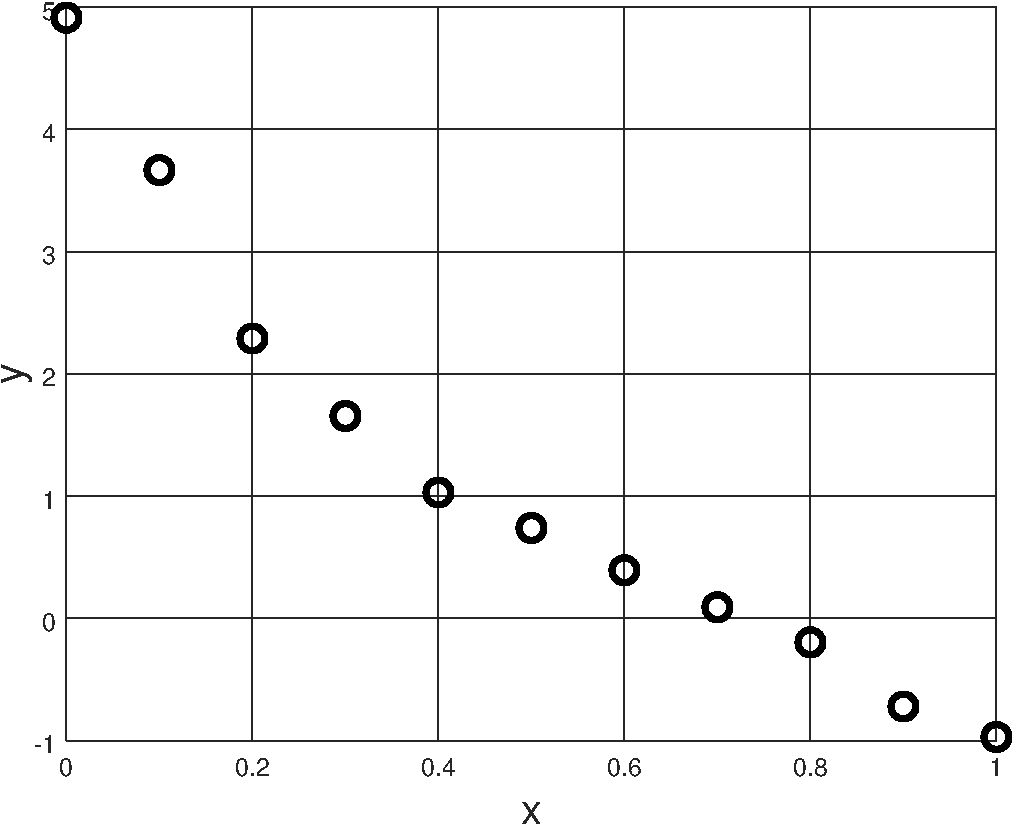
\includegraphics[width=0.5\textwidth]{fitdata}
\end{center}

\medskip
Suppose we believe that this data can be fit by a function of the form
    $$g(x) = c_1 + c_2 x + c_3 e^{-5 x}.$$
If the sense of ``fit'' is that the sum of the squares of the misfits should be as small as possible then we would solve
	$$\min_{c \in \RR^3} f(c)$$
where we define this objective function as\footnote{The overall factor of $1/2$ is a convenience for differentiating.  Which is a hint about the standard algorithms \dots} 
	$$f(c) = \frac{1}{2} \sum_{j=1}^{11} \left(g(x_j) - y_j\right)^2 = \frac{1}{2} \sum_{j=1}^{11} \left(c_1 + c_2 x_j + c_3 e^{-5 x_j} - y_j\right)^2.$$
Note $S=\RR^3$ because there are no constraints on the coefficients $c_i$.

We are \emph{not} finding $x_j$ or $y_j$ values in the minimization process!  We are finding $c_1,c_2,c_3$.  The data values $(x_j,y_j)$ merely determine the objective function.

\bigskip
\item (\texttt{salmon})  \quad Ed and Thomas caught 21 salmon.  Of these, $x_1$ will be eaten fresh, which requires 2 time units per fish.  Then $x_2$ will be vacuum-packed and frozen (3 time units per fish) and another $x_3$ will be smoked and vacuum-packed (4 time units per fish).  Thus the total amount of processing time is $2 x_1 + 3 x_2 + 4 x_3$.  However, at most 2 fish can be eaten fresh before they go bad, and at most 10 fish can be smoked in the time allowed.  Find $x_1,x_2,x_3$ to minimize the total processing time.

This is a constrained minimization problem wherein $x_i$ are numbers of fish, \emph{which must be positive numbers}, and the objective function is the total processing time $f(x) = 2 x_1 + 3 x_2 + 4 x_3$:
	$$\min f(x) \qquad \text{subject to }\quad \begin{matrix} x_1 + x_2 + x_3 = 21 \\ 0 \le x_1 \le 2 \\ 0 \le x_2 \\ 0 \le x_3 \le 10 \end{matrix}$$
Note that the objective function and the constraint functions (e.g.~$g_1(x)=x_1+x_2+x_3$,$g_2=x_1$,\dots) are linear functions.  This is an \emph{linear programming} problem.

The feasible set $S\subset \RR^3$ includes all the constraints:
    $$S = \left\{x \in \RR^3\,\big|\,x_1 + x_2 + x_3 = 21, 0 \le x_1 \le 2, 0 \le x_2, \text{ and } 0 \le x_3 \le 10\right\}.$$
Defining $S$ allows us to put the problem in the standard form ``$\min_S f(x)$''.

\bigskip
\item (\texttt{tsp})  \quad Jill sells amazing widgets that help you learn math.  To sell these devices she plans to visit cities A, F, J, N, W by starting and ending at city S.  Some cities have connecting flights and some do not; the one-way costs of the various flights are shown below in a \emph{graph} with costs (weights) on each connection (edge).  It is clear that she should visit each city exactly once, except for S.

\begin{center}
\vspace{-5mm}
\begin{tikzpicture}[scale=0.9]
\begin{scope}[every node/.style={circle,thick,draw}]
    \node (A) at (-0.5,0) {A};
    \node (F) at (0,3)    {F};
    \node (J) at (2,-1)   {J};
    \node (N) at (-3,3)   {N};
    \node (S) at (3,-3)   {S};
    \node (W) at (3,1)    {W} ;
\end{scope}

\begin{scope}[every node/.style={fill=white},
              every edge/.style={draw=black,very thick}]
    \path (A) edge node {$100$} (F);
    \path (A) edge node {$100$} (J);
    \path (A) edge node {$150$} (N);
    \path (A) edge[bend right=50] node {$250$} (S);
    \path (A) edge node {$150$} (W);
    %\path (F) edge node {$150$} (J);
    \draw[very thick] (F.east) .. controls (3,4) and (6,0) .. (J.east) node[midway] {$150$};
    \path (F) edge node {$200$} (N);
    %\path (F) edge node {$300$} (S);
    \draw[very thick] ([yshift=3mm,xshift=-1mm] F.east) .. controls (4,5) and (7,-1) .. (S.east) node[midway] {$300$};
    \path (F) edge node {$250$} (W);
    \path (J) edge node {$200$} (S);
    \path (J) edge node {$200$} (W);
\end{scope}
\end{tikzpicture}
\end{center}

\medskip
This is an example of the famous \emph{traveling salesperson problem}.  Each possible itinerary is expressible as a seven-letter string like ``SANFWJS.''  If $x$ denotes such a feasible string then we may define the objective function $f(x)$ to be the cost of that itinerary; thus $f(x)$ is defined using the edge weights.  Finding a feasible itinerary for a big enough graph is generally nontrivial; it corresponds to finding a \emph{Hamiltonian cycle}.  One may, however, add in all remaining edges with large weights so that any itinerary $x$ is feasible and has a well-defined cost $f(x)$.

The problem \emph{could} be written in standard form
	$$\min_S f(x).$$
where $S = \{x\,|\,x \text{ is a feasible itinerary}\}$.  However, there is no easy way to describe $S$ by inequalities and equalities as as subset of some Euclidean space $\RR^n$ as above.

In any case, this is a \emph{discrete optimization} problem, not a continuous problem as expected in the course and our textbook.  That is, $S$ is a finite set of feasible itineraries.

\bigskip
\item (\texttt{glacier})  \quad  The shape of an ice sheet on flat bedrock is approximately given by the solution to a constrained optimization problem.  (An ice sheet is just a big glacier.)  Even in the simple case here, the solution to the minimization problem is a \emph{function}.  In fact the objective function $f[u]$ takes a function $u(x)$ as input and produces a single real number.  It is common to call those functions which take functions as input \emph{functionals}.

The feasible set in this specific problem is a set of functions defined on an interval:
    $$S = \left\{v(x) \,\big|\, v(x) \ge 0 \text{ is a differentiable function of } -100 \le x \le 100\right\}.$$
Note $x$ is in kilometers.  The nontrivial constraint is that if $v(x)$ is in $S$ then it is nonnegative; this is because it is a form of the ice thickness (see below).  In contrast to all the above examples, an element of the feasible set $S$ is not a finite list (vector) of numbers, it is a function itself.  This \emph{calculus of variations} problem is infinite-dimensional.

In this specific problem we have a made-up function which defines the rate of total snowfall or melt in a year, the \emph{mass balance} in glaciologist language:
    $$m(x) = \begin{cases} -3 + \frac{6}{90} (x+70), & -70 \le x \le 20, \\
                            3 - \frac{6}{50} (x-20), & 20 \le x \le 70, \\
                           -3, & \text{otherwise}.
             \end{cases}$$
The units of $m(x)$ are meters per year.  This function is graphed below.  Note that it is only snowing where $m(x)$ is positive; everywhere else it is melting.

\bigskip
\begin{center}
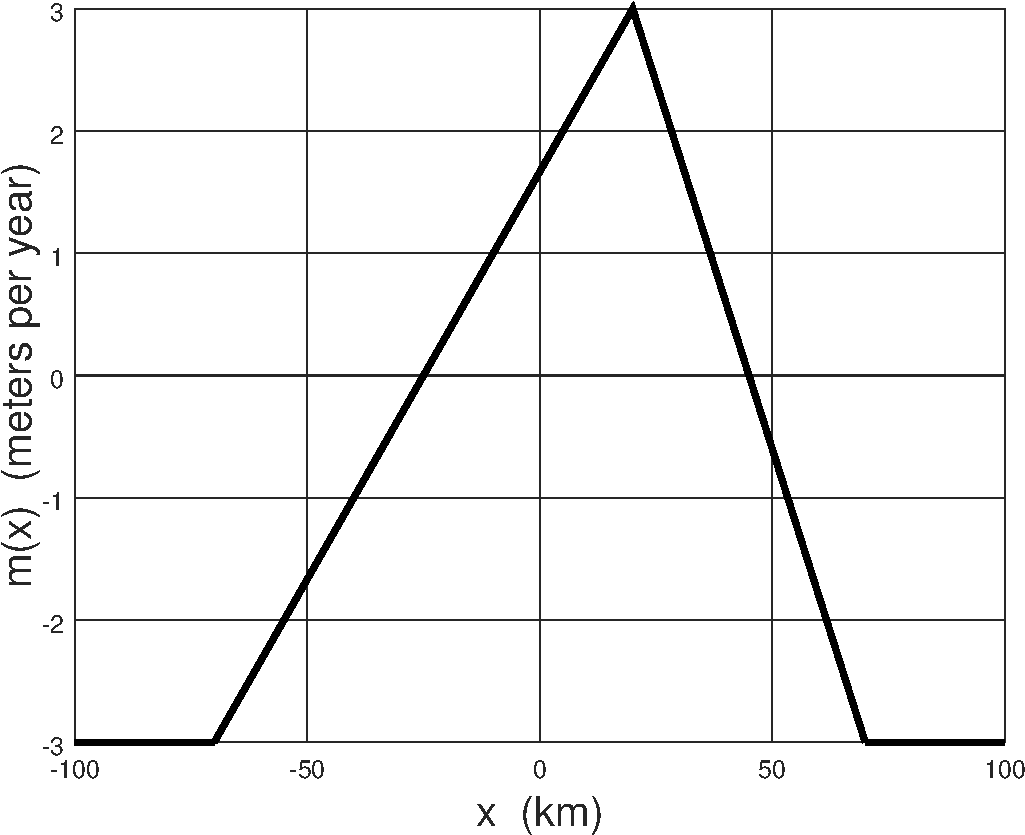
\includegraphics[width=0.5\textwidth]{massbalance}  % see massbalance.m
\end{center}

% regarding how mu is computed:
%>> rho = 910; g = 9.81; p = 4;
%>> A = 1e-16/31556926
%A =    3.1689e-24
%>> Lam = 2 * (rho*g)^3 *A / 5
%Lam =    9.0177e-13
%>> mu = 2 * (rho * g * (p-1) / (2*p))^(p-1) * A / (p+1)
%mu =    4.7554e-14

The objective functional is an integral defined using the data $m(x)$:
    $$f[u] = \int_{-100}^{100} \frac{\mu}{4} \left(u'(x)\right)^4 - m(x) u(x)\,dx$$
Based on other physical constants related to the flow of ice (not shown) we set $\mu = 5 \times 10^{-14}$.  The glacier shape is derived from the solution of the problem
    $$\min_S f[u].$$
Once $u(x)$ is computed we raise it to a power to get the actual height $h(x)$, measured in meters, of the glacier:
    $$h = u^{3/8}.$$  % u^{n/(2n+2)}

Because this problem occurs on an infinite-dimensional feasible set $S$, computer solutions require \emph{discretization}.  (Note that computers can only store finitely-many real numbers.  Storing arbitrary functions on an interval is not possible.)  The easiest way to discretize is to put a grid on the interval $I=[-100,100]$ and only consider functions which are piecewise-linear between the points of this grid.  In that case the derivative $u'(x)$ in the integral for $f[u]$ is computed by a finite difference quotient, namely the slope of the line between points.  Because this way of making the problem finite-dimensional is only an approximation, we want the grid to be as fine as practical given our tools (i.e.~the available optimization algorithms and computer resources).

\end{enumerate}

\end{document}

